\begin{figure}
  \centering
  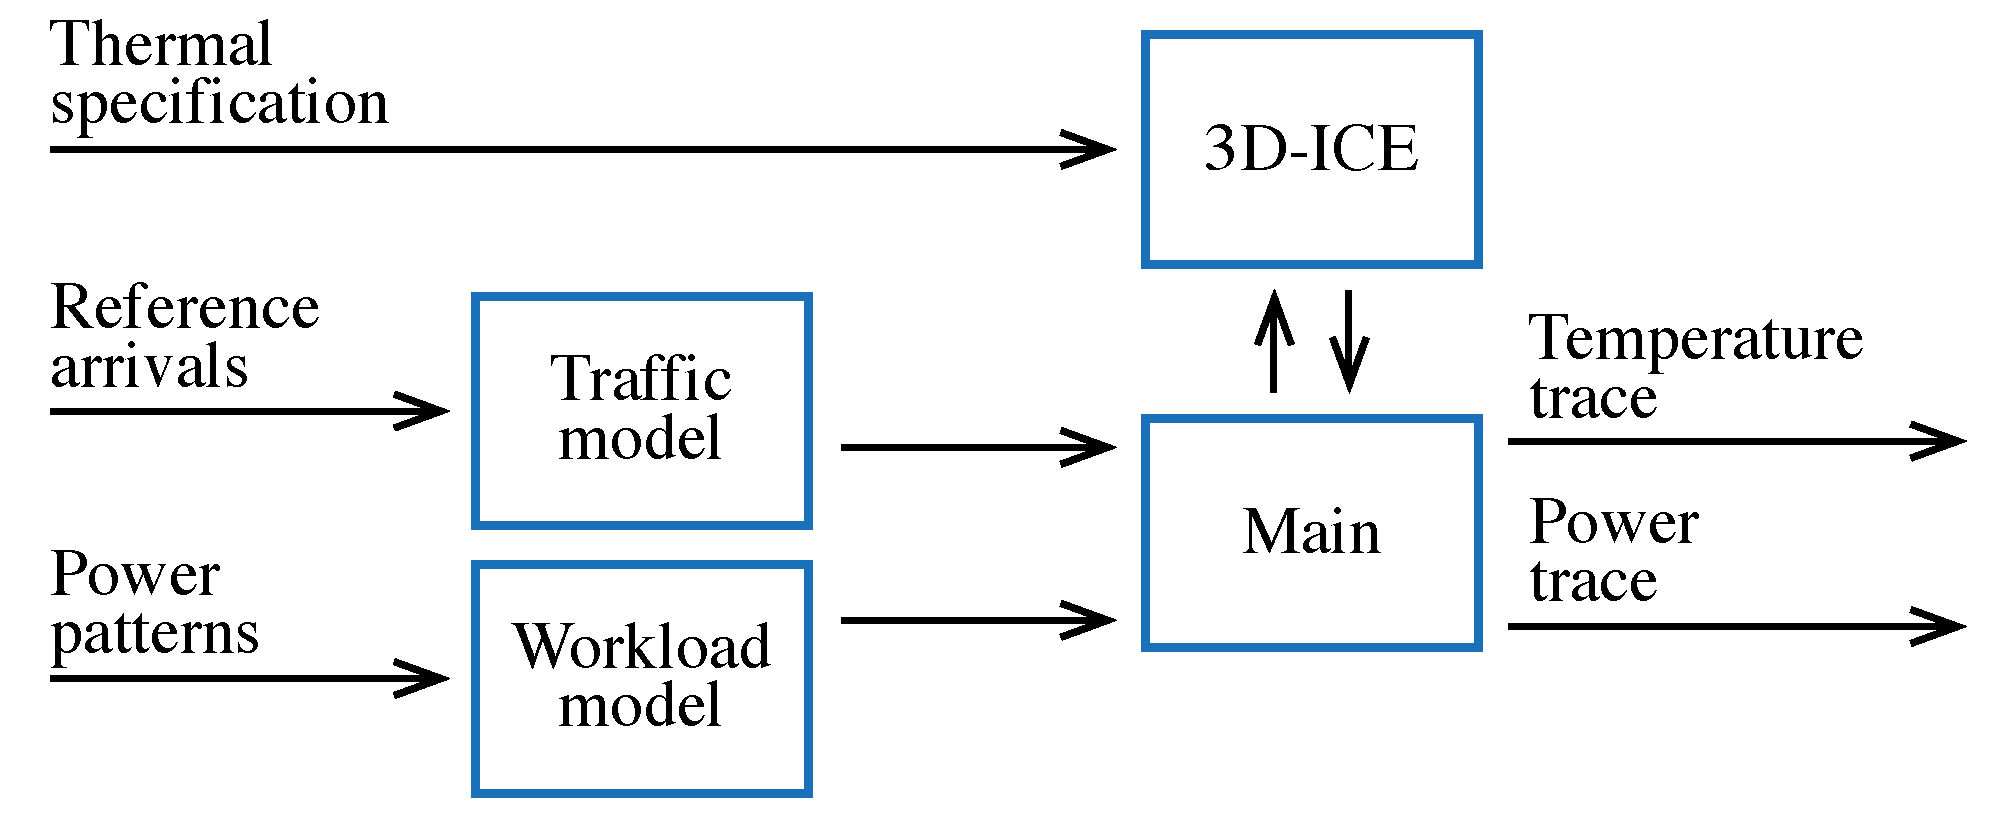
\includegraphics[width=1.0\columnwidth]{include/assets/figures/streamer.pdf}
  \caption{The streaming infrastructure.}
  \flab{streamer}
\end{figure}

The Streamer tool corresponds to the data-synthesis stage, which means that it
is responsible for synthesizing power and temperature data using reference data
as a material for the synthesis; see the module labeled ``Streamer'' in
\fref{methodology}. The structure of the tool is laid out in \fref{streamer}.

Given a traffic pattern and a set of workload patterns, Streamer proceeds as
follows. The traffic pattern is processed as it was described in \sref{traffic},
which results in an adequately configured multifractal wavelet model
\cite{riedi1999}. The model is then used to generate a stream of arrival times.
The arrival times are fleshed out using the workload patterns, which was
explained in \sref{workload}. The result is a stream of jobs, and the whole
operation is referred to as job modeling in \fref{streamer}. The rest follows
\sref{composition}. The job stream is handled by a scheduling policy; in
\fref{streamer}, this policy is a part of the Main module. As the incoming jobs
are being scheduled, the power profile of the system under consideration is
being constructed. The power profile is piped into a temperature simulator (to
be discussed below), which delivers a temperature profile. The synthesized data
(power and temperature) can be fed to the scheduler and/or stored for later
usage. In the latter case, similar to reference data, the output is an SQLite
database.

Let us now outline how temperature simulation is undertaken by Streamer. The
simulation is based on the thermal \sc{RC} model. In this paradigm, a so-called
thermal \sc{RC} circuit representing the system at hand is constructed and then
used to analyze the thermal behavior of the system. The analysis boils down to
solving a system of differential equations. In our case, the solution is based
on a solver leveraging exponential integrators \cite{ukhov2014}. The
construction of thermal circuits is outsourced to either HotSpot
\cite{skadron2004} or \sc{3D-ICE} \cite{sridhar2010} (see \fref{streamer}). We
provide a unified interface for working with the two alternatives.

To summarize, Recorder is used for recording workload patterns, and Streamer
produces streams of power and temperature data. Both closely follow the ideas
presented in \sref{methodology}.
